\section{Table Driven Agent}\label{AI: Agent Programs/Table Driven Agent}


\begin{figure}[H]
    \centering
    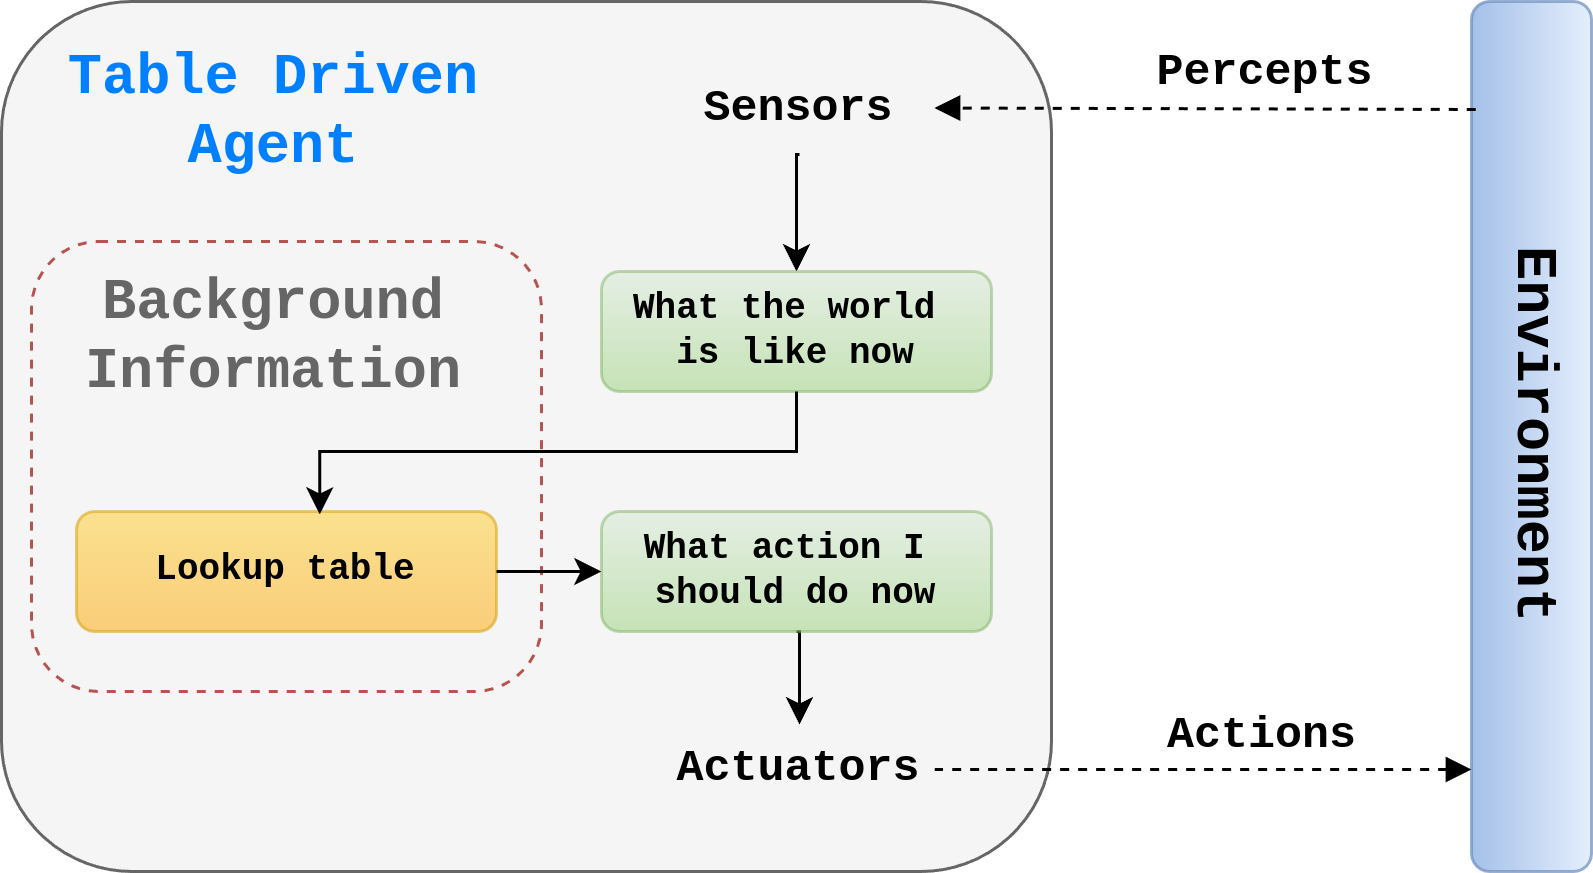
\includegraphics[
        width=0.5\linewidth, 
        height=4cm, 
        keepaspectratio
    ]{images/artificial-intelligence/ai-agents/agents-table-driven-agent.png}
    \caption*{Schematic diagram of a table driven agent. \cite{common/online/tools/draw.io}}
\end{figure}

\begin{longtable}{l l}

$\mathcal{P}$ & set of possible percepts \\

$T$ & lifetime of agent (total number of percepts) \\

\end{longtable}


\vspace{0.5cm}

\begin{enumerate}[itemsep=0.2cm]
    \item Number of entries in table: $
        \dsum_{t=1}^T \dabs{\mathcal{P}}^t
    $
    \hfill \cite{ai/book/Artificial-Intelligence-A-Modern-Approach/Russell-Norvig}
    
    \item Sometimes the number of entries can be ridiculously large number due to the combinations of percepts and length of percept sequence.\\
    \textbf{Example}: Consider the \textit{automated taxi}: the visual input from a single camera comes in at the rate of roughly $27$ megabytes per second ($30$ frames per second, $640 \times 480$ pixels with $24$ bits of color information). This gives a lookup table with over $10^{250,000,000,000}$ entries for an hour’s driving.
    \hfill \cite{ai/book/Artificial-Intelligence-A-Modern-Approach/Russell-Norvig}
    \\
    It means:
    \begin{enumerate}
        \item no physical agent in this universe will have the space to store the table
        \hfill \cite{ai/book/Artificial-Intelligence-A-Modern-Approach/Russell-Norvig}

        \item the designer would not have time to create the table
        \hfill \cite{ai/book/Artificial-Intelligence-A-Modern-Approach/Russell-Norvig}

        \item no agent could ever learn all the right table entries from its experience
        \hfill \cite{ai/book/Artificial-Intelligence-A-Modern-Approach/Russell-Norvig}

        \item even if the environment is simple enough to yield a feasible table size, the designer still has no guidance about how to fill in the table entries
        \hfill \cite{ai/book/Artificial-Intelligence-A-Modern-Approach/Russell-Norvig}

    \end{enumerate}
\end{enumerate}

\vspace{0.5cm}

\begin{algorithm}[H]
    \caption{The \textsc{Table-Driven-Agent} program is invoked for each new percept and returns an action each time. It retains the complete percept sequence in memory. \cite{ai/book/Artificial-Intelligence-A-Modern-Approach/Russell-Norvig}}

    \SetKwFunction{FUNCTION}{\textsc{Table-Driven-Agent}}
    \SetKwProg{Fn}{function}{ returns \normalfont an action}{end}
    \Fn{\FUNCTION{ percept }}{
        \textbf{persistent}:\\
        
        \hspace{0.4cm} $percepts$, a sequence, initially empty\\
        
        \hspace{0.4cm} $table$, a table of actions, indexed by percept sequences, initially fully specified \\
        
        \ \\

        append $percept$ to the end of $percepts$ \\
        
        $action$ $\gets$ \textsc{Lookup}($\ percepts,\ table\ $) \\

        \Return $action$
    }
\end{algorithm}




